\chapter{Webové rozhraní}
\label{kap:webove-rozhrani}

\section{Porovnání s~jinými scénáři}

Mým dílčím cílem je co nejlepší ortografický\footnote{Na pravopis jako takový se důraz
neklade. Ortografickým přepisem myslím standardní zápis.} a fonetický přepis
tisícihodinového korpusu jednoho mluvčího rozděleného do přibližně hodinových
celků. Lidé, kteří se o tyto nahrávky zajímají a chtějí je studovat, představují
potenciál, který mohu využít ke své práci, a zároveň cílovou skupinu, jimž bude
produkt sloužit.

Webová aplikace by tedy měla skloubit tyto dva účely:
\begin{enumerate}
\item{Sloužit uživatelům, aby mohli  materiál co nejlépe konzumovat.}
\item{Navést uživatele, aby vydali co nejkvalitnější příspěvek.}
\end{enumerate}

Neznám žádný projekt se srovnatelným východiskem. Můžeme
však porovnávat jednotlivé aspekty, vyskytující se v~jiných aplikacích.

\subsection{Programy pro přepis}
\label{ssec:diff:trans}

Nástroje určené pro manuální přepis zvukového záznamu do textu představují
typ aplikace, který je mému případu podobný a zároveň rozšířený.
Porovnejme tyto dva úkoly a zpytujme hlavní rozdíly. K~porovnání
vezměme
\begin{enumerate}
\item{
    Transcriber\footnote{trans.sourceforge.net}, klasický svobodný program
    napsaný v~TCL,
}
\item{
    oTranscribe\footnote{otranscribe.com}, svobodný moderní webový přepisovací
    nástroj a
}
\item{
    Transcribe\footnote{transcribe.wreally.com}, komerční webový přepisovací
    nástroj.
}
\end{enumerate}

Každé číslo v~seznamu níže označuje program, pro který platí ten který výrok. Ku
příkladu jen Transcriber umožňuje anotaci mluvčích, proto u druhé položky
stojí pouze číslo (1).



\noindent
\begin{tabularx}{\textwidth}{
    @{\hspace{1.5em}}% Space for left bullet
    >{{\hsize=0.9\hsize}\leavevmode\llap{\textbullet~}\raggedright}% Left bullet + formatting of column
    X% Left column specification
    @{\hspace{0.2em}}
    >{\hsize=0.2\hsize}
    X
    @{\quad\hspace{1.5em}}% Space between columns + right bullet space
    >{\leavevmode\llap{\textbullet~}\raggedright\arraybackslash}% Right bullet + formatting of column
    X% Right column specification
    @{}% No column space on right
  }
  \em{přepisovací programy}: & & \em{moje aplikace}: \\
  jsou optimalizované pro pořízení přepisu od nuly; &
    (1,2,3) &
      vždy vychází z~existence předchozího přepisu; \\

  umožňují anotaci mluvčích; &
    (1) &
      předpokládá, že všechna slova pocházejí od jednoho mluvčího; \\

  nepotřebují kontrolu kvality: uživatel může přepisovat dle libosti a konečným
  měřítkem je jeho vlastní spokojenost; &
    (1,2,3) &
      vyžaduje přesnost přepisu neboť tento je použit pro trénování
      statistických modelů; \\

  zarovnávají na úrovni frází, pokud vůbec; &
    (1)\footnote{
        Transcriber explicitně zarovnává text s mluveným slovem, oproti zbylým
        dvěma, které toliko umožňují přidání časových značek do přepisu.
    } &
      zarovnává na úrovni slov, interně na úrovni fonémů; \\

  točí se kolem uživatele: každý může přepisovat libovolná data; &
    (1,2,3) &
      točí se kolem dat: sbírka nahrávek je středobodem aplikace a přepisovat
      lze pouze ji; \\

  předpokládají, že přepisovat je uživatelův záměr; &
    (1,2,3) &
      předpokládá, že uživatel chce poslouchat, vyhledávat nebo číst
      s~poslechem, a k~přepisu ho nutno motivovat; \\

  nesdílejí data mezi uživateli; &
    (1,2)\footnote{Transcribe podporuje kolaborativní přepis} &
      musí počítat s~kolizemi, kdy více uživatelů upravuje týž úsek. \\
\end{tabularx}

\vspace{5mm}

Navzdory těmto odlišnostem se v~přepisovacím softwaru skrývá mnoho poučného.
Snadnost provádění běžných úkonů, jako pozastavení a obnovení přehrávání či
posun, jsou stěžejní pro uživatelský prožitek {\em (UX)} a tím i pro množství a kvalitu
příspěvků. I způsob synchronního zobrazení textu se zvukem má velký dopad a
v~potenciálních přístupech je značná svoboda pro variaci.

\subsection{Wiki}

Kde se moje aplikace odchyluje od přepisovacích programů, tam do značné
míry připomíná wiki: komunitní platformu, která slouží uživatelům včetně
přispěvatelů, ale kde kvalita příspěvků je podstatná, zatímco samotná
spokojenost přispěvovatelova nemá takovou důležitost.

Jeden podstatný rozdíl oproti wiki je, že wiki je kreativní, kdežto náš úkol je
mechanický. Uživatel má pramálo prostoru pro vlastní invenci: poskytnutí jiného
než doslovného přepisu se vnímá jako chyba.

Populární wiki mají dobrá opatření pro konflikty v~editacích, což je oblast, kde
bych se mohl nechat poučit. Zatím k~tomu ale nebyl důvod, protože pokud vždy
použiji nejnovější verzi každého segmentu, výsledek zůstane konzistentní, i když
segment od uživatele A padne do širšího přepisu od uživatele B.

Nově odeslaný segment přepisu vždy přepíše stávající verzi, ale každý lze
vrátit zpět {\em (undo)}, neboť všechny příspěvky udržuji v~databázi. Lze také
shlukovat příspěvky podle autora či jinak, ale zatím něčeho takového nebylo
zapotřebí.

\subsection{Korpusy}
\label{ssec:setting-corpora}

Tento projekt není prvním, který zahrnuje komunitní péči o korpus. Za zmínku
stojí Manually annotated sub-corpus\cite{ide2010manually}, kde se anotace různého
druhu střádají od dobrovolníků. Dále Wikicorpus\cite{reese2010wikicorpus},
korpus článků z~Wikipedie s~určitou úrovní lingvistické anotace. Můj projekt
by s nimi mohl v~budoucnu dosáhnout značné podobnosti, až se hlavní bod zájmu
stočí od samotného přepisu k~anotaci.

Je zde také CzEng\cite{bojar2008czeng}, česko-anglický paralelní korpus, kde
velká část překladů pochází od dobrovolníků. Podobnost ve východisku je zde
pozoruhodná, neboť v~obou projektech se z~původního materiálu dojde k~derivátu
pomocí počítačového zpracování, přičemž chyby se pak komunitně opravují.
V~případě CzEngu jde o strojový překlad, v~mém o strojový přepis. Nicméně
specifika projektů přinášejí odlišné problémy a diktují odlišné přístupy.

Marge 2009\cite{5494979} zkoumá použití platformy Mechanical Turk k~získání
přepisů mluveného slova. Mihalcea 2004\cite{mihalcea2004building} prezentuje
webové rozhraní pro dezambiguaci významu slov {\em (word-sense disambiguation)} a
zaměřuje se především na ošetření neshod mezi anotátory.

\section{Popis webové aplikace}

Webová aplikace sloužící k~přehrávání a sběru přepisů existuje ve dvou
verzích. Prototyp byl implementován hned za začátku projektu v~roce
2012 a popisuje ho článek Krůza, Peterek 2012\cite{kruuza2012making}. Druhá,
modernější verze začala vznikat na konci roku 2016 a poprvé byla nasazena na
konci září 2017. Tu popisuje článek Krůza, Kuboň
2018\cite{biblio:KrKuSecondGenerationWeb2018}.

\subsection{Prototyp}

První implementace byla založena na přehrávači \textit{jPlayer}, modulu pro
knihovnu \textit{jQuery}, který využívá standard HTML5 s~jeho elementem
\texttt{<audio>} a technologii \textit{Adobe Flash}. Pro~dynamickou odezvu
zobrazených prvků na~změny v~datovém modelu jsem použil knihovnu
\textit{knockout}.

Aplikace měla formu jediné stránky s~rozbalovatelným výběrem nahrávky,
ovládacími prvky přehrávače a třemi řádky přepisu. Při označení části
zobrazeného přepisu se stránka překryla rozhraním pro opravu přepisu, jež zvu
\textit{editačním okénkem}. V~editačním okénku se zobrazilo vstupní pole
(\texttt{<textarea>}) s předvyplněným současným přepisem, ovládací prvky pro
přehrátí odpovídající pasáže, odeslání opraveného přepisu a opuštění editačního
okénka.
Rozhraní prototypu ukazuje obrázek~\ref{fig:prototyp}.

\begin{figure}[htpb]
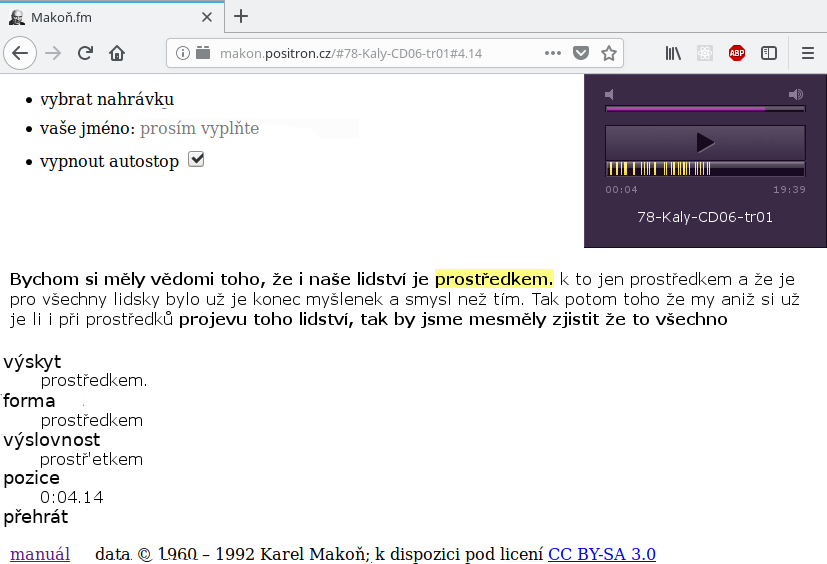
\includegraphics[scale=0.8]{rc/makonfm-cs-1.png}
\caption{První verze webové aplikace.}
\label{fig:prototyp}
\end{figure}

%Každé slovo s~sebou neslo informaci o~svojí pozici v~nahrávce
%s~přesností na~setiny sekundy, výslovnost, zápis, slovníkovou formu, délku ticha
%za~slovem, informaci o~tom, zda bylo manuálně přepsáno nebo automaticky
%rozpoznáno, a v~případě automaticky rozpoznaných slov \textit{confidence
%measure} čili míru jistoty rozpoznání.

%Převod ze~zápisu slova do~jeho fonetické podoby se děje na~základě pravidlového
%algoritmu z~dílny Doc. Pavla Ircinga po~úpravě od~Mgr.~Nina Peterka, Ph.D. Tento
%algoritmus zahrnuje časté výjimky z~českých výslovnostních pravidel, ale
%neobsahuje rozsáhlý výslovnostní slovník cizích slov. Karel Makoň navíc nezřídka
%hovoří o~osobách, jejichž jména se v~mnoha korpusech neobjeví vůbec.

Nad rámec výše popsaných funkcionalit přibyly další na~základě přání uživatelů a
autorovy potřeby:

\begin{itemize}
\item{indikace, do~jaké míry je která nahrávka
přepsána\footnote{\label{fn:not-in-v2}Tato
funkcionalita momentálně není implementována v~nové verzi aplikace.},}
\item{manuální posouvání hranic přepisovaného zvukového
úseku\footnotemark[\getrefnumber{fn:not-in-v2}],}
\item{úprava zápisu slova s~ponecháním výslovnosti,}
\item{identifikace uživatelů včetně sezení, prohlížeče atp.,}
\item{vyhledávání v~přepisech.}
\end{itemize}

Tato původní verze posloužila k~přepsání asi 600 tisíc slov a běžela asi 5 let,
než bylo nutné ji nahradit.

Pro kompletní přepis aplikace se postupně objevilo několik důvodů. Hlavním
z~nich bylo, že původní aplikace mohla jen těžko sloužit pro širokou veřejnost.
Dalším důvodem bylo, že některé kýžené funkce nebylo možné zprovoznit bez
zásadních změn v~provedení. Především šlo o~ekvalizér, čili frekvenční korekci
při poslechu. Akutním důvodem pak byl fakt, že všechny významné prohlížeče
opouštěly podporu Flashe.

\subsection{Základní rysy druhé verze}

Pro novou verzi jsem zvolil technologie React + Redux\cite{abramov2015redux} jako aplikační rámec, Web
Audio API\cite{adenot2013web} jako platformu pro nakládání se~zvukem a Twitter Bootstrap jako základ
pro vzhled prvků. Zdrojový kód píšu v~ECMAScript~6 a o~kompilaci se stará
webpack.

Aplikace sestává z~několika {\em pohledů\footnote{Pohled ve smyslu {\em view}
z~architekturního přístupu {\em model - view - controller}. Podobně jako autoři
frameworku Django, pojmem pohled {\em (view)} míním jednu stránku definovanou cestou
v~URL i s~její funkcionalitou.}}:
\begin{enumerate}
\item{úvodní stránka se seznamem nahrávek, kde každý záznam odkazuje na detailní
pohled,}
\item{detail nahrávky, kde je možné přehrávání a zobrazuje se přepis, který se dá
editovat,}
\item{výsledky vyhledávání, kde každý záznam obsahuje úryvek odpovídající
vyhledávanému dotazu a odkazuje na příslušnou pasáž nahrávky v~detailním
pohledu,}
\item{různé statické podstránky s~obecnými informacemi, manuálem atd.}
\end{enumerate}

Úvodní stránka má
dvousloupcový formát, kde vlevo je rozbalovací seznam kategorií a vpravo
lineární seznam nahrávek. Jednotlivé kategorie jsou pak skrolovacími odkazy
do~pravého sloupce a podle stupně skrolování se příslušná kategorie sama
rozbalí (tzv. {\em scrollspy}).

Pro lepší přehlednost a v souladu s principem {\em separation of concerns} je seznam
nahrávek pouze na~úvodní stránce.

Podrobněji se budu zabývat pouze pohledem detailu nahrávky.
Obrázek~\ref{fig:scn1lab} ukazuje rozhraní v~průběhu přehrávání.
Obrázek~\ref{fig:scn2lab} ukazuje rozhraní při editaci segmentu.

\begin{figure}[htpb]
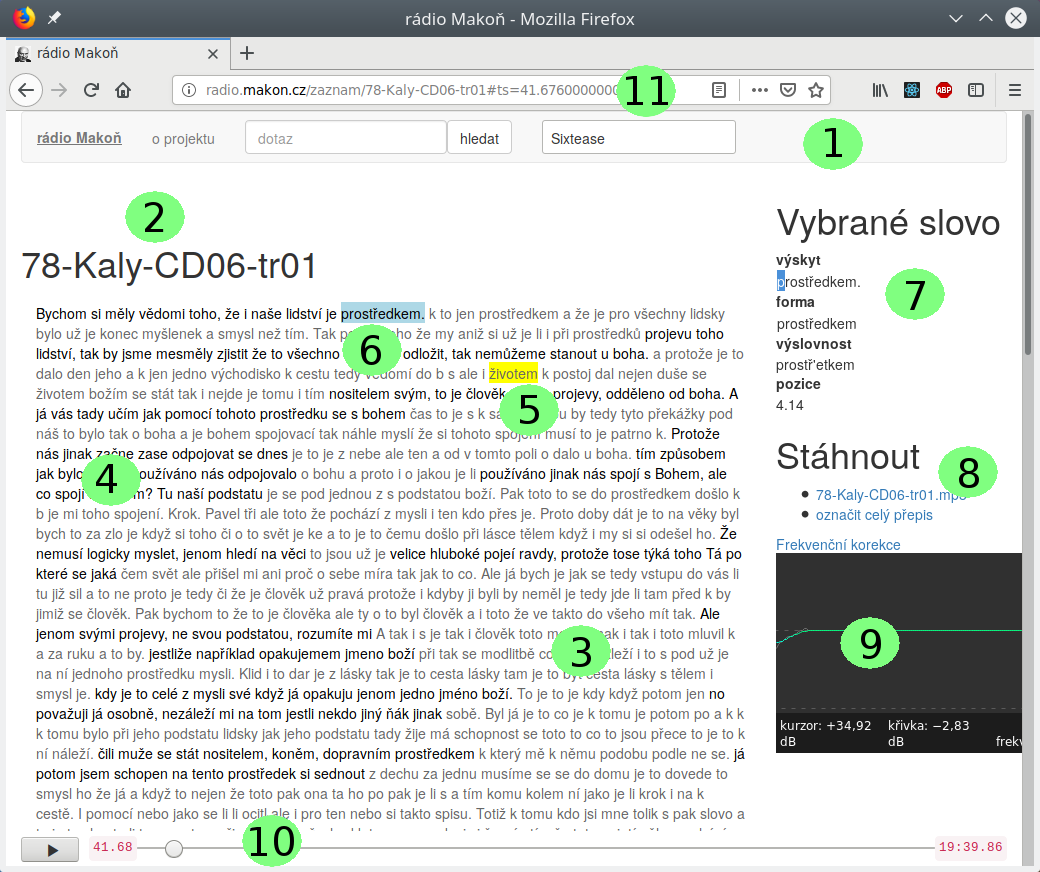
\includegraphics[scale=0.7]{rc/radio-makon-cs-1-lab.png}
\caption{Webové rozhraní při přehrávání.}
\label{fig:scn1lab}
\end{figure}

\textbf{Vysvětliky k~obrázku~\ref{fig:scn1lab}:}
\begin{enumerate}
\item{
    Záhlaví a v~něm
    \begin{itemize}
    \item{jméno aplikace odkazující na úvodní stránku,}
    \item{odkaz na informace o projektu,}
    \item{vyhledávací políčko,}
    \item{vstupní pole pro uživatelovu přezdívku.}
    \end{itemize}
}
\item{Identifkátor nahrávky.}
\item{Automaticky přepsané segmenty v~šedi.}
\item{Manuálně přepsané segmenty v~černi.}
\item{Právě přehrávané slovo zvýrazněné žlutým pozadím.}
\item{Označené slovo zvýrazněné odstínem modři ,,st. regent`` na pozadí.}
\item{
    Informace o označeném slově:
    \begin{itemize}
    \item{
        výskyt: slovo s~kontextuálním velkým písmenem a
        interpunkcí, jak se nachází v~textu
        (navíc právě editované, jak prozrazuje označené iniciální písmeno),
    }
    \item{forma: normalizovaná slovní forma, jak se objevuje ve slovníku,}
    \item{
        výslovnost: český fonetický zápis použité výslovnosti (viz
        podsekci~\ref{ssec:respelling}),
    }
    \item{
        pozice: čas v~sekundách od začátku nahrávky do začátku slova.
    }
    \end{itemize}
}
\item{
    Ukládání:
    \begin{itemize}
    \item{přímý odkaz k~celé nahrávce ve formátu mp3,}
    \item{označení celého přepisu pro snadné vložení {\em (copy-paste)}.}
    \end{itemize}
}
\item{Grafický ekvalizér pro kompenzaci úzkopásmového šumu.}
\item{
    Ovládací prvky přehrávání:
    \begin{itemize}
    \item{tlačítko pro pozastavení / pokračování,}
    \item{současná pozice,}
    \item{posuvník {\em (scrollbar)} přehrávání,}
    \item{celková délka nahrávky.}
    \end{itemize}
}
\item{aktuální pozice reflektovaná v~URL.}
\end{enumerate}

\begin{figure}[htpb]
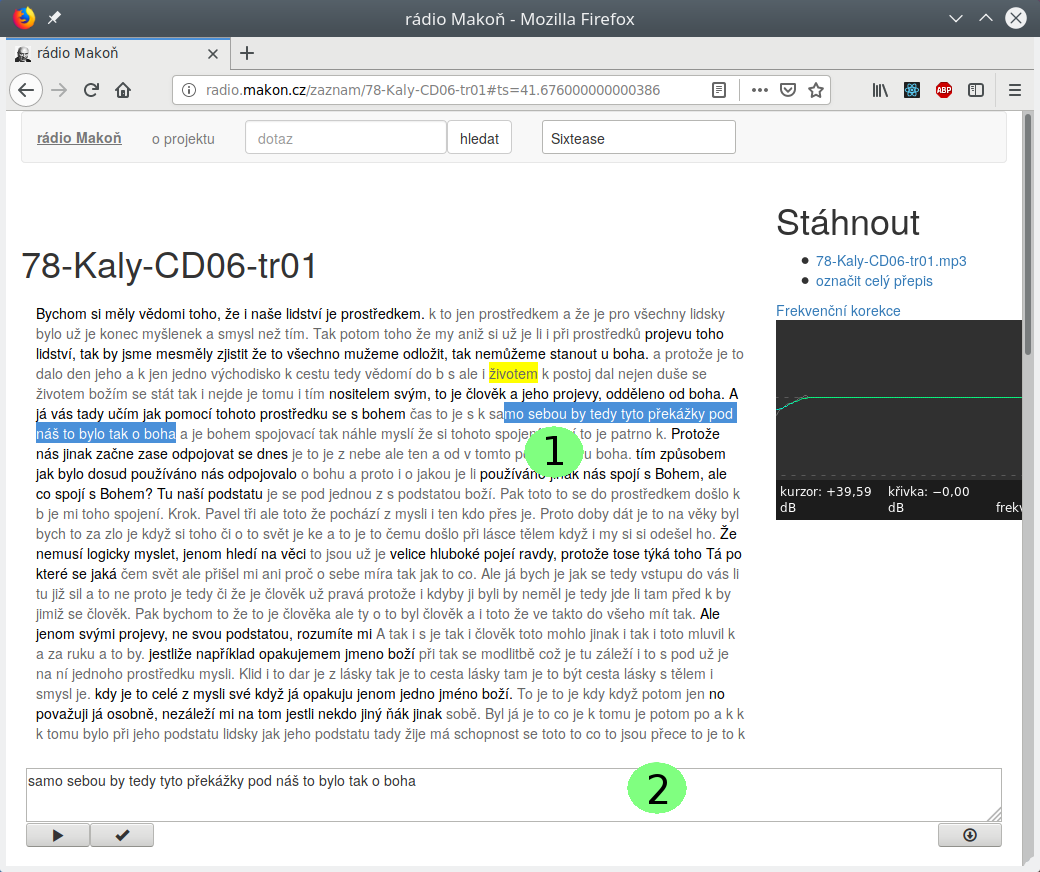
\includegraphics[scale=0.7]{rc/radio-makon-cs-2-lab.png}
\caption{Rozhraní ve stavu editace segmentu.}
\label{fig:scn2lab}
\end{figure}

\textbf{Vysvětlivky k~obrázku~\ref{fig:scn2lab}:}
\begin{enumerate}
\item{
    Označení textového úseku myší definuje segment k~editaci tak, že označené
    části slov se doplní na celá;
}
\item{
    Editační okénko a v~něm:
    \begin{itemize}
    \item{textové pole {\em (textarea)} předvyplněné stávajícím přepisem,}
    \item{tlačítko pro přehrání odpovídajícího segmentu,}
    \item{tlačítko pro uložení,}
    \item{
        tlačítko pro stažení segmentu, které inicializuje operaci uložení
        souboru pro úsek audia odpovídající označenému textu. Syntéza uloženého
        souboru se odehrává v~prohlížeči.
    }
    \end{itemize}
}
\end{enumerate}

Nejčastější úkony mají klávesové zkratky: \texttt{ctrl+mezerník} pro
přehrání / pozastavení a \texttt{ctrl+enter} pro uložení korekce.

\subsection{Zobrazení přepisu}

Mnohý program pro přepisování ukazuje transkript jako vertikální seznam
vyřčených frází,
viz obrázek~\ref{fig:transcriber} pro příklad z~Transcriberu. To připisuji faktu,
že atomickými prvky přepisu jsou uživatelem definované fráze a jejich hranice
jsou spolehlivé. Není na programu, aby je definoval nebo
zpochybňoval. V~mém případě jsou atomickými prvky slova. Ano, jsou zde i věty,
ale segmentace na věty automatickým přepisovačem je velice nespolehlivá, takže
je žádoucí, aby označení a přepsání segmentu, který přesahuje přes hranice věty,
bylo přirozené a snadné.

\begin{figure}[htpb]
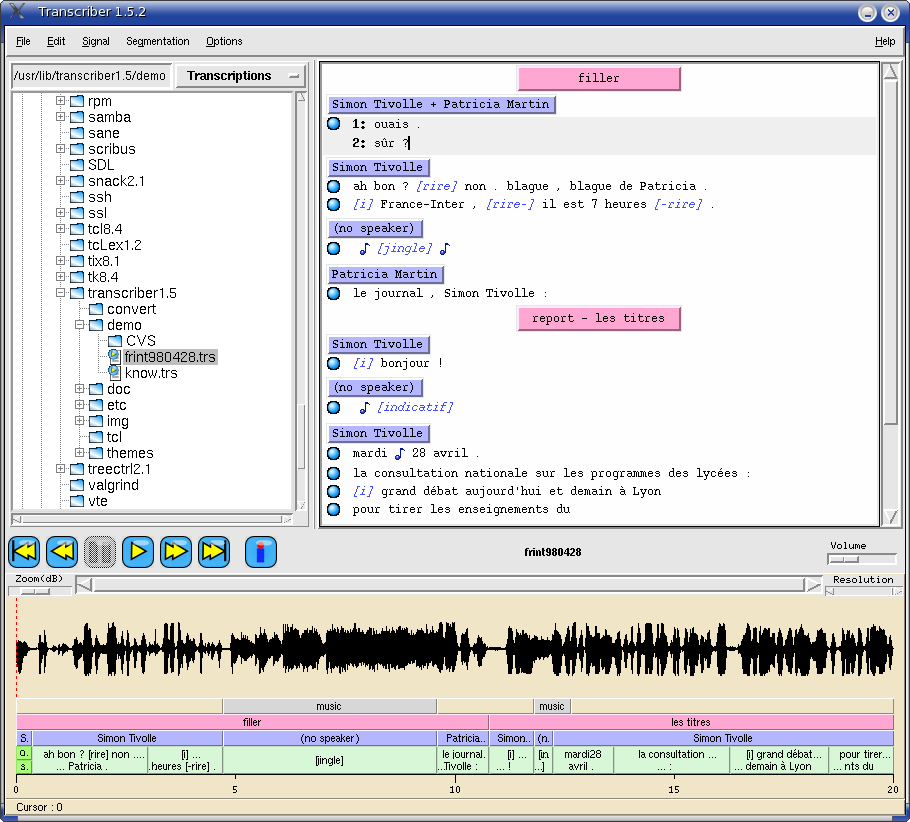
\includegraphics[scale=0.46]{rc/transcriber1.png}
\caption{Uživatelské rozhraní Transcriberu.}
\label{fig:transcriber}
\end{figure}

Toto je jeden z~důvodů, proč zobrazuji přepis v~podstatě jako jeden zalomený
řádek.

\subsection{Problém s~rychlostí}

Na zobrazení přepisu byly kladeny tyto požadavky:
\begin{enumerate}
\item{
    Právě přehrávané slovo aby bylo zvýrazněno.
    \label{feats:item:curword}
}
\item{
    Manuálně přepsané segmenty aby byly jasně odlišené od automaticky
    přepsaných.
    \label{feats:item:manualdistinct}
}
\item{
    Označení neprázdné množiny znaků (krom mezery) myší aby spustilo editační
    mód pro označený text doplněný na celá slova;
    při úspěšném uložení změny aby se tato vmísila do zobrazeného textu.
    \label{feats:item:selectable}
}
\item{
    Kliknutí na slovo aby o~něm vyvolalo zobrazení kontextových informací
    (toto zvu {\em ,,vybrané slovo``}, neb pojem {\em ,,označené slovo``} je již
    obsazen).
    \label{feats:item:clickable}
}
\item{
    Celý přepis aby byl viditelný najednou pro možnost vyhledávání.
    \label{feats:item:showall}
}
\item{
    Stránka aby byla responzivní.
    \label{feats:item:speed}
}
\end{enumerate}

Skloubit tyto požadavky je obtížnější, než by se mohlo zdát. Zejména
responzivita se těžko slučuje s~ostatními body. Proč?

Body~\ref{feats:item:curword} až~\ref{feats:item:clickable} volají po tom, aby
každé slovo bylo obaleno ve vlastním elementu.
Bod~\ref{feats:item:showall} a medián počtu slov v~nahrávce zvíci šesti tisíc
dávají dohromady šest tisíc elementů \texttt{<span>} jen pro statické zobrazení
textu.

Může se zdát, že to není takový problém, ale ovlivňuje to responzivitu a
paměťovou náročnost stránky.

V~původní verzi webové aplikace jsem toto vyřešil obětováním
bodu~\ref{feats:item:showall}. Zobrazovaly se jen tři řádky textu, přičemž právě
přehrávané slovo se vždy drželo v~tom prostředním. Ukazuje to
obrázek~\ref{fig:prototyp}, jen s~tím rozdílem, že právě přehrávané slovo je v~prvním
řádku, poněvadž se přehrává začátek nahrávky. Díky pokroku ve webových
standardech a jejich podpoře ze strany prohlížečů je nyní možné řešení.

\subsection{Řešení}

Můžeme využít šťastného faktu, že ručně přepsaná slova a automaticky přepsaná
slova mají tendenci se shlukovat. Průměrný počet slov v~jednom příspěvku je 7,9.
Navíc drtivá většina takových segmentů bezprostředně navazuje na další ručně
přepsané segmenty.\footnote{Medián počtu shluků je 1 (většina nahrávek nemá
žádné ručně přepsané slovo), maximum je 1109. Medián pouze z~nahrávek, které
obsahují ruční korekce, je 8.}
Z~toho plyne, že obalení každého souvislého shluku manuálně či automaticky
přepsaných slov do zvláštního HTML elementu nepředstavuje problém. Tím se řeší
bod~\ref{feats:item:manualdistinct}.

Bod~\ref{feats:item:selectable} lze implementovat s~použitím metody objektového
modelu dokumentu ({\em DOM}) \texttt{document.selection} a objektů
\texttt{Range}, které umožňují nalézt nejhlubší HTML elementy a pozice v~jejich
textu, kde začíná a končí označený úsek. Díky tomu, že délka slov je známa, mohu
z~označeného úseku dovodit odpovídající slova v~přepisu.

Body~\ref{feats:item:curword} a~\ref{feats:item:clickable} se dá implementovat
dvěma způsoby: Buďto zabalením přehrávaného a vybraného slova do zvláštního
elementu anebo vykreslením zvýrazňujícího obdélníku na pozadí slova.

Výhodou obalení slov elementem by byla větší robustnost a menší náchylnost
k~chybám. Nicméně neustálé změny v~DOMu při přehrávání s~potenciálními častými
operacemi {\em reflow}\footnote{Při operaci reflow prohlížeč přepočítává pozice
všech elementů a překresluje je.} hovoří proti tomuto řešení. Nalézt přesné
pozice slova a vykreslení obdélníku přesně pod ním\footnote{Pod ním na ose Z.
Přes něho na osách X, Y.}, vyhnout se chybám v~pozicování a udržet
obdélník na správném místě i po změně velikosti okna či odskrolování, to je
dozajista výzva, nicméně přesto jsem zvolil tuto cestu. Navýšení výkonnosti pro
běžné používání převažuje potenciální chyby v~okrajových případech, najmě když
eventuální chyby nejsou kritické a zmizí při dalším přehrávání.

Efektivitu repozicování obdélníku podporuje i fakt, že se dají dopředu spočítat
souřadnice všech slov najednou a pak je přepočítat jen ve dvou případech:
1) při zřídkavé události změny velikosti okna a
2) když se opravený segment vkládá do zobrazeného přepisu a je tedy
nutno souřadnice přepočítávat pouze pro slova, která jsou v~dokumentu za
vloženým segmentem.

Dalo by se optimalizovat dále a zastavit přepočet
v~momentě, kdy se nějakému slovu nezmění horizontální souřadnice. Pak by stačilo
připočíst rozdíl ve vertikální souřadnici všem následujícím slovům. Jinými
slovy, pokud jeden řádek zůstane stejný, pak i všechny pod ním.

\subsection{Vizuální odlišení manuálního a automatického přepisu}

Jak je vidět na obrázku~\ref{fig:scn1lab}, vykresluje se automatický přepis
v~šedé barvě a manuální v~černé. Proč jsem zvolil rozlišení barvou a ne standardním
versus tučným písmem? Za prvé, standardní písmo je optimalizované pro čtení.
Tučné písmo je na to, aby bodově zvýrazňovalo úseky. Když se použije na dlouhé
pasáže, působí těžkopádně. Automatický přepis obsahuje mnoho chyb, takže nedává
smysl ho optimalizovat pro ideální četbu.

Je ještě jeden praktický důvod. Když se varianty písma liší pouze v~barvě,
nikoliv ve velikosti, a když segment automatického přepisu je beze změny odeslán
jako zkorigovaný, pak jeho vložení do textu nezpůsobí reflow, což šetří
výpočetní kapacitu a napomáhá responzivitě. Může se to zdát jako okrajový
případ, ale domnívám se, že identifikace správně automaticky přepsaných slov je
legitimní způsob přispívání, tak proč ho neoptimalizovat?

Automaticky přepsané úseky balím i tak do elementů
\texttt{<span>} a manuálně přepsané do elementů \texttt{<b>}, protože potom se
rozlišení zachová při zkopírování textu z~webové stránky do textového editoru
podporujícího formátování.

\subsection{Web Audio API}

Přechod na~tuto technologii umožnil některé pokročilé funkce, avšak za~relativně
vysokou cenu. Web Audio API je standard pro~pokročilé zpracování zvukového
signálu v~prohlížeči. Základním konceptem je graf procesních uzlů, které mají
vstup a výstup a mohou se libovolně propojovat. K~dispozici jsou zdroje zvuku
jako oscilátory nebo přehrávače streamů, souborů (tag \texttt{<audio>}) a dat
v~paměti (\texttt{AudioBuffer}) a efekty jako zesílení, dynamická komprese, či
mixování kanálů.

Velká výhoda Web Audio API oproti elementu \texttt{<audio>} je možnost přesného
časování až k~jednotlivým samplům. Přehrávání výseku odpovídajícího označenému
textu se proto nemusí provádět pomocí velice nepřesného časovače
\texttt{setTimeout}.

Bez~Web Audio API by také nebylo možné provádět frekvenční korekci při poslechu,
čili mít tzv. \textit{ekvalizér}. Ten je zapotřebí, protože některé nahrávky
mají v~určitém frekvenčním pásmu silný šum, jehož odstranění je s~ekvalizérem
snadné a komfort poslechu se tak razantně zvýší.

Další funkcí, kterou Web Audio API umožňuje, je stahování úseků. Označením
přepsaného textu se definuje úsek nahrávky a ten je možné uložit bez~dalšího
síťového přenosu. Tato funkce však vyžaduje, aby nahrávka byla dekódovaná
v~paměti. Vzhledem k~tomu, že nahrávky mají běžně i hodinu a půl, trvá její
stažení a dekódování opravdu dlouho a navíc prohlížeč kvůli tomu spotřebuje přes
gigabyte operační paměti.

Jsou plány na~to, aby Web Audio API umožnila dekódovat jen část
nahrávky\footnote{github.com/WebAudio/web-audio-api/issues/1305}, avšak
palčivost problému mne přiměla nečekat, viz následující sekci.

Díky tomu, že Web Audio API umožňuje přehrávání binárních dat z~proměnné
v~paměti, nabízí se dekódovanou nahrávku uložit na~persistentní úložiště
uživatelova počítače a při opětovné návštěvě stránky data místo stahování odsud
nahrát.

Moderní prohlížeče poskytují několik bran k~úložišti na~místním disku.
Nejtradičnějšími jsou bezesporu \textit{cookies}, které jsou však pro ukládání
objemnějších dat zcela nepoužitelné. Velice slibnou se jeví
\textit{localStorage}, umožňující ukládání párů klíč-hodnota. I zde však
narážíme na~příliš omezující kvóty. Kupříkladu Firefox ji má na 10MB, přičemž
potřeba je asi 1GB. Dalším kandidátem je \textit{File System API}. Tento
standard pro~izolovaný souborový systém k~dispozici webové aplikaci je zcela
ideálním řešením -- dá se zde i explicitně požádat o~konkrétní diskovou kvótu a
uživatel tak má volbu bez nutnosti práce programátora webové aplikace. Kamenem
úrazu je zde však podpora, která se momentálně omezuje pouze na Google Chrome.

Existuje ještě standard \textit{IndexedDB API}, který má uspokojivou
podporu a uložení gigabytu dat je s~ním možné, byť ne zaručené. S~využitím
abstrahující knihovny \textit{Dexie} jsem proto skrz tento standard ukládání
implementoval. Pro uživatele, kteří delší dobu pracují na jedné a téže nahrávce,
se tím přináší velká úspora času a přenesených dat. Nicméně s~rozdělením
nahrávek na segmenty přestala být potřeba ukládat nahrávky aktuální.

\section{Rozdělení nahrávek na úseky}
\label{sec:segmenty}

Vzhledem k~tomu, že ani v~roce 2019 není kurzorový přístup ke zvukovým datům
skrze Web Audio API v~dohlednu, a jak odrazující dopad má nutnost
stahovat a dekódovat celou nahrávku aspoň při jejím prvním načtení, nezbylo mi,
než změnit způsob, jakým jsou nahrávky uloženy. Toto je popsáno v~článku Krůza 2019/1\cite{kruza2019restructuring}

Nahrávky jsou uloženy v~několika instancích pro různé účely:

\begin{enumerate}
\item{na backendovém serveru ve formátu MFCC pro nucené zarovnávání,}
\item{v~repozitáři LINDAT ve formátu FLAC za účelem archivace a bádání,}
\item{na {\em CDN}\footnote{content delivery network} ve formátu mp3 za účelem přímého stažení uživatelem,}
\item{taktéž na CDN ve formátech OGG/Vorbis a mp3 pro webové rozhraní.}
\end{enumerate}

Pouze poslední jmenovanou instanci je žádoucí ukládat tak, aby každý soubor byl
jen tak velký, aby jeho stažení a dekódování trvalo únosně dlouho. V~ostatních
případech je lépe zachovat uložení, kde jedna nahrávka odpovídá většinou
jedné straně kazety či jednomu průchodu pásky z~kotouče na kotouč. Třetí a čtvrtá
instance však navzdory rozdílnému účelu sdílejí tatáž data. Bylo proto nutné je
duplikovat.

\subsection{Délka segmentů}

Délka úseků, na které nahrávky rozděluji, ovlivňuje, jak dlouho se každý segment
bude stahovat a dekódovat.  Čas stahování a dekódování segmentu, který obsahuje
slovo, na němž je kurzor při prvním požadavku o~přehrávání, je roven zpoždění od
uživatelské akce k začátku přehrávání. Podle internetového periodika
UXMovement\cite{foursecondrule}, začíná uživatel po čtyřech sekundách čekání
upouštět od předchozího záměru. Podle článku Nielsen Norman
Group\cite{websiteresponsetimes} je hranice únosnosti 10 sekund.

Pokud budou úseky příliš dlouhé, jejich stahování a dekódování zabere příliš
mnoho času. Na druhou stranu s každým předělem vnášíme do přehrávání bod, kde se
úseky nalepují a může tam vyvstat artefakt. Také s~každým segmentem se pojí
extra HTTP request s~nezanedbatelnou režií.

Jako vhodný kompromis se jeví segmenty o délce 30 - 120 sekund. Velikost
dvouminutového segmentu je v~komprimovaném jednokanálovém formátu při vzorkovací
frekvenci 24kHz kolem 0,6MB a na Intel Core2 o 2,5GHz se dekóduje asi 1,6
sekundy.

\subsection{Metody hledání bodů předělu}

Vhodným výběrem bodů předělu můžeme omezit dopad případných artefaktů
způsobených nepřesným navázáním. Ideálním by bylo dělit nahrávky v~momentech
ticha. Ne vždy jsou momenty ticha každé dvě minuty, proto z momentů ticha
ustupme k~požadavku pauzy v~řeči. Hovořit dvě minuty bez nádechu hraničí
s~nemožností. Potýkáme se tedy s~úlohou nalézt pauzy v~řeči. Jednak je třeba
ujasnit, podle jakého klíče budeme pauzy vybírat, a jednak, jak je budeme přesně
hledat.

Hledat pauzy v~řeči lze různými způsoby. Nejspolehlivější a nejnáročnější je
manuální označování pauz. Pokoušel jsem se o~to sám a dosáhl jsem rychlosti
přibližně čtyřnásobku rychlosti přehrávání, tedy jeden zapsaný bod předělu za
třicet sekund.

Další velice spolehlivou metodou je hledání podle predikovaných pseudofonémů
ticha v~zarovnaném přepisu. Tuto metodu jsem mohl namnoze použít, neboť
k~většině nahrávek mám automatický nebo i manuální přepis.

Tam, kde pořízení přepisu nebo jeho automatické zarovnání selhalo, lze použít
detekci ticha prostou akustickou analýzou. Tato metoda je velice náchylná
k~chybám v~případě nahrávek s~malým poměrem signálu k~šumu, a těch je v~korpusu
Karla Makoně mnoho.

Kde nepomůže ani metoda detekce ticha, což se pozná podle toho, že detekované
pauzy jsou příliš daleko od sebe nebo naopak zabírají valnou část nahrávky,
nezbývá, než určit body předělu ve fixních intervalech, nehledě na to, že jich
mnoho padne doprostřed slova.

Pokusy dvě metody vyloučily: Manuální hledání bylo příliš neefektivní. Kromě mne
se dalších asi pět dobrovolných anotátorů o~tento úkol pokusilo a došla jim
trpělivost po nule až deseti minutách označkovaného materiálu. I na některé
nahrávky, u nichž přepis selhal, šlo detekci pomocí
zarovnaného přepisu použít.
Rozdělily se na menší části, tyto se přepsaly, zpravidla
s~malou úspěšností. Tento přepis opět v~některých případech selhal, ale
většina takové nahrávky byla nějakým přepisem pokryta. A jakkoliv nekvalitní
takový přepis byl, právě dlouhé mezery mezi slovy se nalezly s~uspokojivou
přesností. Krátké úseky, na nichž selhalo rozpoznávání řeči, byly pak příliš
obtížné i pro detekci pomocí ticha. Jednalo se o úseky bez řečových událostí,
nebo s~extrémním šumem.


Celkový počet různě získaných bodů předělu shrnuje
tabulka~\ref{tab:splitpoints}\footnote{Vysoký počet předělů fixní délkou je způsoben tím, že
k~některým nahrávkám jsem doposud nepořídil zarovnaný přepis s~vyznačením délky
ticha.}.

\begin{table}[htpb]
\begin{center}
\begin{tabular}{|l|l|}
\hline
metoda získání & počet použitých \\
\hline
manuálně & 0 \\
podle zarovnaného přepisu & 60424 \\
podle detekce ticha & 0 \\
fixní délkou & 22043 \\
celkem & 82467 \\
\hline
\end{tabular}
\caption{Počet bodů předělu podle metody jejich získání.}\label{tab:splitpoints}
\end{center}
\end{table}

\subsection{Výběr bodů předělu}

V~metodě určování bodů předělu pomocí fixního intervalu jsem zvolil délku
šedesáti sekund. Výše rozvádím, že to je délka přijatelná, a další
optimalizací tohoto parametru jsem se nezabýval.

Zajímavější je situace u~hledání pomocí zarovnaného přepisu. Zde se jedná
o~programátorský úkol, kde na vstupu máme posloupnost slov vyskytujících se
v~přepisu nahrávky, z~nichž každé s~sebou krom své formy a výslovnosti nese
informaci, kde začíná, a pokud obsahuje na konci ticho, pak kde začíná
pseudofoném ticha a jak je dlouhý. Vstup tedy můžeme redukovat na posloupnost
párů čísel, kde první vždy udává počátek ticha a druhé jeho konec. Na výstupu
očekáváme posloupnost časových pozic, které rozdělují nahrávku na úseky o~délce
nejméně 30 sekund, nejvýše 120 sekund, a které jsou uprostřed co nejdelších
tich.

Povšimněme si, že úloha nemá řešení, pokud je nahrávka kratší třiceti sekund. To
ovšem v~mluveném korpusu Karla Makoně nenastává a ani v~opačném případě by to nevadilo,
protože takovou nahrávku bychom nechali v~jednom souboru.

Úloha nemá řešení i v~případě, kdy mezi dvěma sousedními tichy
je rozestup větší než 120 sekund. Takový případ nastává, když je samotné
detekované ticho velmi dlouhé. Tyto případy jsem řešil manuální úpravou.

Hledaný algoritmus se zdá být typickým příkladem pro dynamické programování:
Nalezneme ideální rozdělení nahrávky, která obsahuje jen první slovo, a poté
přidáváme slova, načež na základě dosavadního řešení a nového slova řešení
rozšiřujeme.

Je ale i jednodušší varianta: Začneme s~množinou všech tich a iterujeme přes ně
od nejkratší po nejdelší. Ticho z~množiny odebereme, pokud sloučením sousedních
segmentů nevznikne segment delší než 60 sekund. Přes vybraná ticha znova
iterujeme a ticho odebereme, jestliže jeden z~jeho sousedů má méně než 30
sekund.

Zbylá množina tich splňuje počáteční podmínky, pokud to je vzhledem ke vstupním
datům možné. Algoritmus je jednoduchý na naprogramování a má milou
lineární složitost.

\subsection{Pojmenování souborů}

Jsou-li vybrány body předělu, mohou se nahrávky podle nich rozdělit a výsledné
segmenty uložit na disk. Zde vyvstává otázka, jak rozdělit soubory do adresářů a
jak je pojmenovat. Způsob uložení souborů hraje svou roli, jak dokládá i
Reppen\cite{reppen2010building}. Zvolil jsem tento formát:

\texttt{{\em{}ID}/{\em{}format}/{\em{}ID}--from-{\em{}ZACATEK}--to-{\em{}KONEC}.{\em{}PRIPONA}}

tedy například

\texttt{88-04A/ogg/88-04A--from-1155.27--to-1211.53.ogg}.

Důvody jsou tyto: Není praktické z~důvodu omezení mnoha souborových systémů mít
příliš mnoho souborů v~jednom adresáři. Používám proto rozdělení do adresářů podle
identifikátorů nahrávek. Že formát je právě podadresář identifikátoru a ne třeba
nadadresář, je arbitrární. Obojí by bylo možné, stejně jako mít soubory všech formátů
v~jednom adresáři a odlišovat je jen příponou.

Zopakovat identifikátor nahrávky i v~názvu souboru jsem se rozhodl proto, aby
případný zatoulaný soubor mohl být snáze identifikován. Díky tomu, že se do
názvu souboru uvede začátek i konec úseku v~rámci nahrávky, je zajištěno, že název
souboru přesně popisuje jeho obsah. Oproti tomu např. lineární číslování by při
změně bodů předělu vedlo k~tomu, že jeden název souboru by byl totožný pro různé
úseky v~různých verzích korpusu. To by mohlo vést k~problémům s~cachováním.
Odvozování identifikátorů na základě binárního obsahu souboru, např. pomocí
kontrolních součtů, by vedlo k~nutnosti změnit identifikátory při každé
změně komprese apod., ačkoliv slyšitelný rozdíl by třeba nebyl žádný.

Pokud by při současném řešení došlo ke změně bodů předělu, by se nové i staré úseky musely
uchovávat v~jednom adresáři, a až by všechny reference na staré úseky byly
vyhlazeny z~paměti cache všech klientů, mohly by se staré smazat. Jedinou
nevýhodou je, že staré a nové úseky by byly pomíchané v~jednom adresáři, a proto
by se musely při mazání explicitně vyjmenovat.

\subsection{Překryv úseků}

Při testování se ukázalo, že vyřízneme-li pomocí programu \texttt{sox} úsek
zvukového souboru, výsledný soubor skončí přehrávání o~několik desetin sekundy
dříve. Jako by chybělo posledních několik set samplů. Příčinu tohoto fenoménu
zatím neznám. Kompenzoval jsem jej tím, že jsem každý úsek prodloužil o~půl
sekundy. Následkem toho bylo potřeba upravit přehrávání tak, aby každý úsek
skončil tehdy, až dohraje jeho metadaty daná délka, nikoliv až do skutečného
vyčerpání zvukových dat.


\section{Použití aplikace}

Aplikace {\em znamená} použití. Použitelnost je tedy klíčovým faktorem pro její hodnocení.

\subsection{Expertíza uživatelů}

Přepis, který pořizuji, je na hranici toho, co se dá nazvat lingvistickou
anotací dat. V~naší požehnané části světa, kde podíl analfabetů je zanedbatelný,
můžeme přepis mluveného slova stěží nazvat odbornou prací. Na druhou stranu zajistit, aby
přepis přesně odpovídal mluvenému projevu
\begin{itemize}
\item{jakožto vyjádření vyřčených slov a jejich významu,}
\item{na fonetické úrovni foném na foném}
\item{a na časové ose}
\end{itemize}
je za hranicemi toho, co se dá očekávat od nevyškoleného uživatele.

Lingvistická anotace dat obecně vyžaduje zaškolené pracovníky. Podíváme-li se
např. na Pražský závislostní korpus, můžeme si povšimnout, že od anotátorů
vzešla taková úroveň expertízy, že se stali spoluautory\cite{hajivc2005complex}.

{\em Crowdsourcing}, přístup založený na komunitní spolupráci nebo zapojování
dobrovolníků, nabývá na popularitě při získávání hodnot, které by jinak byly
neúnosně drahé, viz podsekci~\ref{ssec:setting-corpora}. Nicméně např.
Maekawa\cite{maekawa2000spontaneous} popisuje tvorbu
mluveného korpusu spontánní japonštiny s~využitím placených anotátorů.

Ve většině případů je kvalita pro anotaci dat velmi důležitá, proto je aspoň
nějaká kontrola nezbytná, ať už je odbornost anotátorů jakkoliv vysoká. Je
zřejmé, že čím méně expertízy na straně anotátorů, tím silnější kontroly je
zapotřebí.

Běžnou metodou kontroly kvality je mezianotátorská shoda. To má obrovskou
nevýhodu v~tom, že každá část dat musí být anotována aspoň dvakrát, což snižuje
výtěžnost nejméně o 50\%.

Ještě jeden důvod hovoří proti jejímu použití v~případě tohoto projektu. Webová
aplikace je dělaná pro lidi, kteří chtějí poslouchat Makoňovy nahrávky
z~vlastního zájmu a jejich přínos pro kvalitu přepisu je spíše vedlejším
produktem. Nebylo by snadné přesvědčit je, aby si vybrali právě nahrávku, kterou
už někdo jiný přepsal.

Naštěstí lze implementovat automatický mechanismus, který uživatelům dopomůže
k~vyšší kvalitě příspěvků.

Webová aplikace vychází z~předpokladu, že a-priori existuje nějaký přepis ke
každé nahrávce, takže uživatelův příspěvek je vlastně korekcí. Každý příspěvek
má formu nahrazení textového segmentu jiným. Jelikož přepisy jsou zarovnány
s~audiem na časové ose, víme také, jakému přesně úseku nahrávky daný text
odpovídá.

Dále se vychází z~existence akustického modelu pro nahrávky, viz kapitolu~\ref{kap:asr}.

Díky těmto dvěma prvkům mohu provést nucené zarovnání {\em (forced alignment)} textového úseku
s~audiem. V~případě selhání zarovnání můžeme předpokládat, že úsek byl přepsán
chybně, příspěvek odmítnout a dát tím uživateli zpětnou vazbu. Jelikož
jednotlivé úseky odpovídají akustickému modelu v~různé míře, dochází k~falešně
pozitivním i negativním vyhodnocením.

Falešně pozitivní případ (když systém přijme chybný přepis) představuje skutečný
problém, protože chyba vstoupí do trénovacích dat. Falešně negativní případy
mohou uživatelé často obejít tím, že správný, leč odmítnutý přepis, pošlou
znova, rozdělený do kratších částí. Touto metodou by se pochopitelně mohlo také
podařit vnutit systému nesprávný přepis. Nepředpokládám však na straně uživatelů
zlou vůli.

Krom zachycení chybného přepisu slouží nucené zarovnání k~přesné synchronizaci
na časové ose. Tento prvek zcela chybí prakticky ve všech programech pro přepis,
viz porovnání v~podsekci~\ref{ssec:diff:trans}.

\subsection{Pořízení fonetického přepisu}
\label{ssec:porizeni-fonetickeho-prepisu}

Fonetický přepis je nezbytný pro trénování akustického modelu. Pořizuje se
provedením nuceného zarovnání na každý {\em ortograficky} manuálně přepsaný segment. Pokud je více
výslovnostních variant, automaticky se zvolí ta, která lépe odpovídá akustickému
modelu. Na to je potřeba pořídit výslovnostní varianty každého slova. Používám
kombinaci pravidlového převodníku inspirovaného Psutkou et
al. (2004)\cite{psutka2004development} a dynamického výslovnostního slovníku. Dynamický
výslovnostní slovník je seznam alternativních výslovností každého slova, který
se rozšiřuje s~používáním aplikace.

Manuál k~aplikaci vyzývá uživatele, aby text přepisovali podle standardního
českého pravopisu, ale při zachování maximální věrnosti vyřčených slov, tedy aby
nekorigovali
\textipa{/\textltailn{}a:k/}
%\fontspec{DoulosSIL} /ɲaːk/ \normalfont
na {\em nějak}, nýbrž
přepsali doslova jako {\em ňák}. Fonetický slovník obsahuje časté výslovnostní
varianty, např. počáteční
%\fontspec{DoulosSIL} /v/ \normalfont
\textipa{/v/}
ve slovech
začínajících na
%\fontspec{DoulosSIL} /o/\normalfont,
\textipa{/o/},
tedy
%\fontspec{DoulosSIL} /vopit͡si  voblʊdnoʊ̯ /   \normalfont 
\textipa{/vopi\t{ts}i voblUdn\t*{oU}/}
mohou přepsat jako {\em opici obludnou}.

V~případě slov s~nestandardní výslovností, tedy primárně cizích slov, se od
uživatelů žádá, aby slovo přepsali foneticky. Teprve po úspěšném zarovnání a
integraci do přepisu mohou slovu nastavit kýženou pravopisnou formu. Toto je
jeden z~mála případů, kdy se od uživatele chce něco nekonvenčního.

Když je pravopisně chybný, fonetický zápis poslán, pak pokud projde fází
nuceného zarovnání, integruje se do zobrazeného přepisu. Datová reprezentace
každého slova sestává z~těchto prvků:
\begin{enumerate}
\item{Výskyt:
    slovo, jak se vyskytuje v textu, včetně zachování velkých a malých písmen a
    přilehlé interpunkce.
}
\item{Slovní forma:
    slovo, jak je zaneseno v~jazykovém modelu a ve výslovnostním slovníku.
    (Slovní forma se odvozuje algoritmicky z~výskytu převedením do malých písmen
    a odstraněním neabecedních znaků. Z~toho plyne, že interpunkce a všechny
    neabecední znaky jsou vždy součástí přilehlého slova a nikdy netvoří token
    samy o sobě.)
}
\item{Výslovnost:
    seznam fonémů.
}
\item{Časová značka:
    vzdálenost počátku slova od počátku nahrávky v~sekundách s~přesností na dvě
    desetinná místa.
}
\item{Manuálně přepsané:
    pravdivostní hodnota odlišující manuálně přepsaná slova od automaticky
    přepsaných.
}
\item{Confidence measure:
    míra jistoty, se kterou bylo slovo predikováno (týká se pouze automaticky
    přepsaných slov).
}
\item{Ticho:
    začátek a délka ticha, pokud se za slovem vyskytuje.
}
\end{enumerate}
Jakmile je slovo součástí přepisu, lze upravit jeho {\em výskyt}, tedy jak se
jeví v~textu. Nyní může uživatel vložit správnou ortografickou formu odchylující
se od českých pravidel výslovnosti.

To má za následek přidání dvojice {\em slovní forma - výslovnost} do dynamického
výslovnostního slovníku. Tento úkon je proto nutné provést jen jednou pro každé
slovo. Pokaždé, když na toto slovo libovolný uživatel narazí znova, stačí zadat jeho
ortografickou formu a správná výslovnost se dovodí automaticky.

Například při prvním setkání se jménem {\em George} je potřeba je přepsat jako
{\em džordž}. Poté lze tomuto slovu změnit výskyt na {\em George}, čímž se do
dynamického výslovnostního slovníku tento pár zápis - výskyt přidá. Všechny
další výskyty tohoto jména se pak mohou přepisovat jako {\em George} a správnou
výslovnost systém aplikuje automaticky.

\subsection{Fonetický zápis}
\label{ssec:respelling}

Přese všechny výhody reprezentace fonémů podle systému PACal se nejedná o
pratktický zápis výslovnosti pro laické Čechy. Díky jednoduchému, povětšinou
deterministickému mapování mezi fonémy a grafémy je fonetický zápis, nebo jak
se tento mechanismus označuje anglicky, {\em pronunciation respelling},
v~češtině něčím přirozeným a spolehlivým. Není ani potřeba explicitního dělení
slabik, jako tomu je u angličtiny
(Wikipedie\footnote{https://en.wikipedia.org/wiki/Pronunciation\_respelling}
udává příklad {\em ``Diarrhoea`` is pronounced DYE-uh-REE-a}).
Že tato technika je přirozenou pro všechny rodilé mluvčí češtiny se základním vzděláním,
postuluji jako fakt bez podpůrného výzkumu a zakládám to čistě na vlastní
zkušenosti.

Převod z~fonetického zápisu do PACal obstarává zmíněný převodník, viz
podsekci~\ref{ssec:porizeni-fonetickeho-prepisu}. Je ale zapotřebí i opačného
směru, aby se uživateli mohla dát možnost zkontrolovat, zda slovo, které
přepsal, se uložilo se správnou výslovností.

Za tímto účelem jsem vytvořil javascriptový modul pro převod mezi seznamem
fonémů a českým fonetickým zápisem. Popsán je v~článku Krůza 2018\cite{biblio:KrPhoneticTranscription2018}.

Algoritmus je jednoduchý. Ve většině případů jeden foném odpovídá jednoznačně
jednomu písmenu ve fonetickém přepisu. Výjimky jsou tyto:
\begin{enumerate}
\item{Foném \texttt{x} se píše {\em ch}.}
\item{Fonémy \texttt{dz, dzh} se píší {\em dz, dž}.}
\item{Dvojhlásky \texttt{aw, ew, ow} se píší {\em au, eu, ou}.}
\item{
    Sekvence \texttt{c h, o u, a u, e u, d z, d zh} se píší
    {\em c'h, o'u, a'u, e'u, d'z, d'ž}.
    Budiž však poznamenáno, že sekvence \texttt{c h} je ryze hypotetická, ana
    porušuje spodobu znělosti.
}
\item{
    Neznělou zvýšenou alveolární vibrantu označuji {\em ř'}.
}
\item{
    Palatální a labiodentální nazála se píší {\em n', m'}.
}
\item{Ticho na konci slova ve fonetickém přepise nevyznačuji.}
\end{enumerate}

Modul umožňuje obousměrný převod, ačkoliv v~aplikaci je zapotřebí jen směr ze seznamu fonémů do
fonetického zápisu určeného pro člověka. Uživatel sice může explicitně vyznačit
neznělé {\em eř} oproti znělému, či posloupnost hlásek {\em o}, {\em u} oproti
dvojhlásce {\em ou} pomocí apostrofu. Za osm let provozu však tohoto nebylo ani
jednou potřeba.

Podotýkám, že ve výstupu převodníku do fonetického zápisu se nikdy nevyskytují
sekvence {\em di, ti, ni, dě, tě, ně}. Palatální souhlásky jsou vždy vyjádřeny
explicitně a např. sekvence {\em n i} se vždy vyjádří jako {\em ny}.

V tabulce~\ref{tab:priklady-fonetiky} uvádím několik příkadů slov s~jejich výslovností a fonetickým zápisem, jak jej
produkuje algoritmus, pokud na vstup dostane příslušnou výslovnost ve formátu
PACal.

\begin{table}[htpb]
%\fontspec{DoulosSIL}
\begin{center}
\begin{tabular}{|l|l|l|l|}
\hline
slovo   & výslovnost v~IPA               & výsl. v~PACal  & fonetický zápis \\
\hline
nic     & \textipa{\textltailn{}I\t{ts}} & nj i c         & ňic \\
kdo     & \textipa{gdo}                  & g d o          & gdo \\
disk    & \textipa{dIsk}                 & d i s k        & dysk \\
dřít    & \textipa{d\|'ri:t}             & d rzh ii t     & dřít \\
třít    & \textipa{t\|'{\r*{r}}i:t}      & t rsh ii t     & tř'ít \\
auto    & \textipa{\t*{aU}to}            & aw t o         & auto \\
nauka   & \textipa{naUka}                & n a u k a      & na'uka \\
džbán   & \textipa{\t{dZ}ba:n}           & dzh b aa n     & džbán \\
odžít   & \textipa{odZi:t}               & o d zh ii t    & od'žít \\
odznak  & \textipa{o\t{dz}nak}           & o dz n a k     & odznak \\
podzemí & \textipa{podzEmi:}             & p o d z e m ii & pod'zemí \\
noc     & \textipa{no\t{ts}}             & n o c          & noc \\
tento   & \textipa{tEnto}                & t e n t o      & tento \\
hangár  & \textipa{HaNga:r}              & h a ng g aa r  & han'gár \\
samba   & \textipa{samba}                & s a m b a      & samba \\
tonfa   & \textipa{toMfa}                & t o mg f a     & tom'fa \\
\hline
\end{tabular}
\caption{Příklady algoritmicky získaného fonetického zápisu.}\label{tab:priklady-fonetiky}
\end{center}
\end{table}
%\normalfont

Použití apostrofu pro rozlišení víceznačností a zvláštností není stoprocentně
intuitivní a představuje další bod, kde je zapotřebí uživatele zaškolit, aby
tuto funkcionalitu dokázal patřičně využívat.

\subsection{Vyhodnocení kvality přepisů}

Jak stojí výše, webová aplikace krom jiného slouží pro získání kvalitního
zarovnaného přepisu od laických uživatelů. Pokusím se vyhodnotit, do jaké míry
se to podařilo.

Pro vyhodnocení kvality přepisů nemám žádná referenční data. Naopak, přepisy
používám jako gold standard, tedy referenční data pro trénování akustického ba i
jazykového modelu. Lze se však namátkou podívat na několik vzorků a získat tak
představu o tom, jak si systém vede.

Jednou z~věcí, které můžeme posoudit, jsou přijetí a odmítnutí příspěvků
zarovnávačem. Celkem z~109640 pokusů o zarovnání jich 3419 bylo odmítnuto, což
je 3,12\%. Manuálně jsem prošel 20 náhodně vybraných odmítnutých pokusů a
přišel jsem k~těmto číslům:
\begin{itemize}
\item{
    V~\textbf{11} případech se jednalo o falešná negativa, u nichž přepis byl
    správný a měl být přijat,
}
\item{
    ve \textbf{4} případech byly příčinou odmítnutí akustické nedostatky jako
    např. šum,
}
\item{
    ve \textbf{4} případech se jednalo o pravdivá negativa způsobená chybně
    zvolenými hranicemi segmentu a
}
\item{
     v \textbf{1} případě se jednalo o pravdivé negativum způsobené chybným
    přepisem.
}
\end{itemize}

Ve 25\% tohoto malého vzorku tedy zarovnávač splnil svoje validační
poslání, předšed tomu, aby se do trénovacích dat dostal chybný vzorek. V~55\%
případů selhal a byl jen překážkou v~práci a ve zbývajících 20\%
případů sice odmítl validní přepis, ale zabránil tomu, aby se do trénovacích dat
dostal defektní vzorek, na což se dá dívat v~pozitivním světle.

Dá se také vyhodnotit scénář s~nestandardní výslovností. Za tím účelem jsem
z~dynamického výslovnostního slovníku vybral 4 nadějné záznamy a prohlédl si
příspěvky, které je obsahují. Tabulka~\ref{tab:eval-pronunc} uvádí pro každý
z~nich správnou ortografickou formu, chybnou výslovnost získanou převodníkem,
správnou výslovnost a konečně možný fonetický zápis. Ke každému údaji je uvedeno,
kolikrát se objevil v~manuálně přepsaných datech.

\begin{table*}[htpb]
%\fontspec{DoulosSIL}
\begin{center}
\begin{tabular}{|l r|l r|l r|l r|}
\hline
psaná forma  & \# & \makecell{chybná\\ výslovnost}
                                             & \# & \makecell{správná\\ počeštělá\\ výslovnost}
                                                                               & \# & fonetický zápis
                                                                                                   & \# \\
\hline
Moody        &  2 & \textipa{moPodI}         &  0 & \textipa{mu:dI}            &  4 & múdy, můdy   & 2 \\
Descartes    &  2 & \textipa{dEs\t{ts}artEs} &  0 & \textipa{dEka:rt}          &  4 & dekárt       & 2 \\
Weinfurter   & 30 & \textipa{vEInfUrtEr}     & 13 & \textipa{vajnfUrtr}        & 19 & vajnfurtr    & 2 \\
Michelangelo &  6 & \textipa{mIxElaNgElo}    &  2 & \textipa{mIkElaN\t{dZ}Elo} &  4 & mikelandželo & 0 \\
\hline
\end{tabular}
\caption{Příklady nestandardní výslovnosti v~manuálních přepisech.}
\label{tab:eval-pronunc}
\end{center}
\end{table*}

\begin{table*}[htpb]
\begin{center}
\begin{tabular}{|l|r|r|}
\hline
 & foneticky správně & foneticky chybně \\
\hline
ortograficky správně & 25 & 15 \\
\hline
ortograficky chybně & 6 & 0 \\
\hline
\end{tabular}
\caption{Správnost fonetické a ortografické reprezentace cizích slov na základě
tabulky~\ref{tab:eval-pronunc}.}
\label{tab:pronunc-rate}
\end{center}
%\normalfont
\end{table*}

Z~tabulky~\ref{tab:pronunc-rate} je patrno, že většina případů je správně jak
po stránce fonetické, tak po stránce pravopisné. Pouze asi ve 13\% případů je
uchována pravopisně nesprávná forma. To připisuji tomu, že uživatelé, kteří jsou
si této problematiky vědomi, většinou celý proces dokončí a formu upraví.

Na druhou stranu téměř třetina případů vykazuje ponechání chybné fonetické
reprezentace. To představuje závažný problém alespoň z~dvou úhlů pohledu:
Dokazuje se tím, že nucené zarovnání selhává při zachycení zcela odlišné
výslovnosti, a zároveň se touto cestou dostávají do trénovacích dat špatné
vzorky.

Jednou z~patrných příčin je, že dynamický slovník rozpoznává pouze exaktně
shodná slova. V~jednom souboru je například vidět, jak všechny výskyty slova
{\em Weinfurter} mají výslovnost správně, zatímco ostatní formy, jako např. {\em
Weinfurterovi}, chybně.

Krom toho jistě budou hrát roli neinformovanost a roztržitost uživatelů, což se
jim dá mít těžko za zlé, vzhledem k~tomu, jak náročná činnost na soustředění se
od nich chce.

Případ nesprávné ortografické formy oproti tomu nepředstavuje tak závažný
problém. Může sice ztížit vyhledávání, ale to lze provést na výslovnosti,
už nyní manuálně, a v~případě potřeby automatizovat.

Čtvrtá kombinace fonetického zápisu a špatné výslovnosti se pochopitelně
nevyskytuje.

\normalfont 

\section{Backend}

Popsaná webová aplikace, která je uživatelským rozhraním, spoléhá na aplikační
rozhraní {\em (API)}, odkud dostává aktuální přepisy, kam posílá příspěvky od
uživatelů, a na hosting, odkud stahuje zvukové soubory.

\subsection{API}

Backendová aplikace má formu HTTP serveru s~následujícími koncovými body.

\begin{enumerate}
\item{
    Odeslání manuálního přepisu segmentu
    \begin{itemize}
    \item{cesta: \texttt{/subsubmit}}
    \item{metoda: \texttt{POST}}
    \item{
        parametry:
        \begin{itemize}
            \item{\texttt{trans} (řetězec): přepis jak jej vložil uživatel,}
            \item{\texttt{filestem} (řetězec): identifikátor nahrávky,}
            \item{\texttt{start} (desetinné číslo): pozice začátku přepsaného segmentu od začátku nahrávky v~sekundách,}
            \item{\texttt{end} (desetinné číslo): pozice počátku přepsaného segmentu, ditto,}
        \end{itemize}
    }
    \item{
    odpověď při úspěchu: \begin{alltt}\{
  success: 1,
  filestem: {\em řetězec},
  start: {\em desetinné číslo},
  end: {\em desetinné číslo},
  data {\em (seznam zarovnaných slov)}: [ 
    \{
      fonet: {\em řetězec},
      wordform: {\em řetězec},
      occurrence: {\em řetězec},
      humanic: 1, {\em (znamená, že je manuálně přepsané)}
      timestamp: {\em desetinné číslo}, {\em (pozice začátku slova)}
      slen: {\em desetinné číslo}, {\em (délka ticha, jen když > 0)}
    \},
    {\em ...}
  ]
\}\end{alltt}
    }
    \item{odpověď při selhání: \texttt{\{ message: {\em řetězec} \}}}
    \end{itemize}
}
\item{
    Požadavek na seznam přepisů
    \begin{itemize}
      \item{cesta: \texttt{/init}}
      \item{metoda: \texttt{GET}}
      \item{
        odpověď:\\ \texttt{jsonp\_init(\{ subversions => \{ {\em identifikátor} => {\em verze}, {\em ...} \} \})}
      }
    \end{itemize}

    Verze se inkrementuje při každém příspěvku. Slouží k~tomu, aby se mohly cachovat
    přepisy, ale aby se cache nepoužila, pokud někdo přepis změnil.
}
\item{
    Inicializace sezení
    \begin{itemize}
      \item{cesta: \texttt{/req}}
      \item{metoda: \texttt{POST}}
      \item{parametry:
        \begin{itemize}
          \item{\texttt{username} (řetězec),}
          \item{\texttt{session} (řetězec, nepovinný),}
        \end{itemize}
      }
      \item{odpověď: \texttt{\{ status: "OK" \}}}
    \end{itemize}

    Slouží k~detekci začátku práce na přepisech pro účely sledování času
    potřebného k~přepisům.
}
\item{
    Požadavek statistiky, z~jaké části je která nahrávka přepsána
    \begin{itemize}
      \item{cesta: \texttt{/humpart}}
      \item{metoda: \texttt{GET}}
      \item{odpověď: \begin{alltt}\{
  {\em identifikátor}:
      human: {\em celé číslo - počet manuálně přepsaných slov}
      total: {\em celé číslo - celkový počet slov}
  {\em ...}
\}\end{alltt}
      }
    \end{itemize}

    Tento endpoint momentálně nová verze webového rozhraní nepoužívá, byl
    zamýšlen jako vodítko pro uživatele při výběru nahrávky pro přepis a
    pro navození soutěživého ducha.
}
\item{
    Změna atributů zarovnaného slova v~přepisu \\
    \begin{itemize}
        \item{cesta: \texttt{/saveword}}
        \item{metoda: \texttt{POST}}
        \item{parametry:
            \begin{itemize}
                \item{\texttt{wordform} (řetězec): slovo malými písmeny bez interpunkce,}
                \item{\texttt{occurrence} (řetězec): slovo, jak se vyskytuje v~textu,}
                \item{\texttt{fonet} (řetězec): fonémy oddělené mezerou, zavržený
                parametr, používá se endpoint \texttt{subsubmit},}
                \item{\texttt{timestamp} (desetinné číslo): pozice začátku slova od
                začátku nahrávky v~sekundách,}
                \item{\texttt{stem} (řetězec): identifikátor nahrávky,}
            \end{itemize}
        }
        \item{odpověď: \texttt{\{ success: 1 \}}}
    \end{itemize}
    Editace slova v~přepisu. Používá se, když slovu, které je foneticky správně
    přepsané a zarovnané, je potřeba změnit ortografickou formu, např. u cizích
    slov, doplnit interpunkci atp.
}
\end{enumerate}

Veškerá komunikace je kódována v~UTF-8.

Koncový bod \texttt{subsubmit} pro přijetí (nebo odmítnutí) přepisu úseku
nahrávky, provede na straně serveru nucené zarovnání přijatého přepisu
s~odpovídajícím úsekem audia. Z~toho důvodu je nutné, aby na serveru byly
nainstalované nástroje \texttt{HVite} a \texttt{HCopy} z~HTK, dále aby tam byla
kompletní sada nahrávek ve formátu MFCC a akustický model. Bohužel se zdá, že
nucené zarovnání funguje v~HTK pouze s~monofonémovým modelem, takže přesnost
v~rozlišování přesných a chybných příspěvků není optimální.

\subsection{Ukládání dat}

API používá databázi PostgreSQL pro ukládání příspěvků, metadat k~nim a nepravidelných
výslovností. Ke každému příspěvku se ukládá
\begin{itemize}
\item{samotný přepis,}
\item{identifikátor nahrávky,}
\item{časové rozmezí odpovídajícího úseku nahrávky,}
\item{zda byl přepis přijat,}
\item{datum a čas přispění,}
\item{přezdívka autora, pokud ji vyplnil,}
\item{identifikátor sezení,}
\item{verze prohlížeče.}
\end{itemize}

Každé uživatelské sezení má taktéž svůj záznam a ukládá se proň totéž, co pro
příspěvek, krom příspěvku samotného.

Dále se v~databázi ukládají verze přepisů, které se inkrementují při každém
příspěvku.

Poslední věcí v~databázi je fonetický slovník. Ten slouží ke sběru fonetických
reprezentací slov s~nestandardní výslovností, jejichž výslovnost a psanou formu
poskytují uživatelé.

Přepisy se ukládají trojitě. Primárně na serveru v~souborech ve formátu {\em
JSONP}\footnote{JSON with padding -- JSON obalený do JavaScriptové funkce.}.
Tyto se při každé změně zálohují na externí cloudové úložiště. Do třetice se
denně a na požádání exportují do HTML, které je přístupné z~CDN.
CDN slouží též k~servírování samotných nahrávek.


\section{Budoucí práce}

Webovou aplikaci je potřeba dále zdokonalovat s~ohledem na UX. Rád bych
snížil potřebu zaškolení uživatele zpřehledňováním ovládacích prvků a
integrací vhodného systému nápovědy. Dále chci odstranit nutnost označovat
úsek, aby ho člověk mohl opravit.
Metody zvýšení použitelnosti webu lze čerpat např. z~knihy Jana Řezáče Web
ostrý jako břitva\cite{rezac2016web}.

Nucené zarovnání je nyní založeno na programu \texttt{HVite} ze sady HTK a
využívá jednotného monofonémového akustického modelu pro všechna data. Je
potřeba tento stav napravit, aby se zvýšila přesnost rozpoznání validního úseku
od vadného. Dosáhne se toho buďto natrénováním různých akustických modelů pro
různé skupiny nahrávek nebo použitím jiného programu.

Nabízí se julius. Ten sice neoplývá funkcionalitou nuceného zarovnání s~daným
textem, ovšem dokáže provést nucené zarovnání s~textem, který predikuje. Pomocí
vhodně zvolené restriktivní gramatiky by se tak nuceného zarovnání dalo
dosáhnout. Práh pro odmítnutí by se pak mohl nastavit pomocí confidence measure.
